\documentclass[11pt,a4paper]{article}

% ===============================================================================
% PREAMBLE & PACKAGES (Strict adherence to spec)
% ===============================================================================
\usepackage[margin=1.5cm, top=2cm, bottom=2cm]{geometry}
\usepackage{fontspec}
\setmainfont{Latin Modern Roman}
\setmonofont{Latin Modern Mono}
\usepackage{unicode-math}
\setmathfont{Latin Modern Math}
\usepackage{xcolor}
\usepackage{tikz}
\usetikzlibrary{shapes.geometric, arrows.meta, positioning, calc, fit, decorations.pathreplacing}
\usepackage[most]{tcolorbox}
\usepackage{tabularx, booktabs, array, multirow}
\usepackage{enumitem}
\usepackage{fancyhdr}
\usepackage{titlesec}
\usepackage{tocloft}
\usepackage{hyperref}

% ===============================================================================
% HYPHENATION & SPACING RULES
% ===============================================================================
\hyphenpenalty=10000
\exhyphenpenalty=10000
\sloppy

% ===============================================================================
% COLOR PALETTE (Strict adherence to spec)
% ===============================================================================
\definecolor{myred}{RGB}{196,30,58}       % section headings
\definecolor{mydark}{RGB}{30,30,50}       % body text
\definecolor{mygreen}{RGB}{14,120,80}     % definition boxes
\definecolor{myteal}{RGB}{0,130,140}      % formula boxes, diagrams, subsection headings
\definecolor{myamber}{RGB}{180,100,0}     % example boxes
\definecolor{mypurple}{RGB}{100,30,160}   % exam/viva boxes
\definecolor{myblue}{RGB}{25,90,170}      % hyperlinks/diagrams
\definecolor{mygray}{RGB}{246,247,249}    % tikzbox background
\definecolor{mgframe}{RGB}{180,185,200}   % tikzbox border
\definecolor{watermark}{RGB}{145,150,170} % footer watermark

\definecolor{hdrred}{RGB}{250,232,235}
\definecolor{hdrgreen}{RGB}{220,244,233}
\definecolor{hdrteal}{RGB}{220,242,244}
\definecolor{hdramber}{RGB}{253,242,215}
\definecolor{hdrpurple}{RGB}{238,228,255}
\definecolor{hdrblue}{RGB}{235,242,250}

% ===============================================================================
% TCOLORBOX STYLES (Standard MAKAUT Spec)
% ===============================================================================
\tcbset{
  tikzbox/.style={colback=mygray, colframe=mgframe, boxrule=0.6pt, arc=4pt,
    left=8pt, right=8pt, top=6pt, bottom=6pt,
    colbacktitle=mgframe, coltitle=mydark, fonttitle=\small\bfseries},
  defbox/.style={colback=hdrgreen, colframe=mygreen, boxrule=0.8pt, arc=4pt,
    left=9pt, right=9pt, top=6pt, bottom=6pt,
    colbacktitle=mygreen, coltitle=white, fonttitle=\small\bfseries},
  formulabox/.style={colback=hdrteal, colframe=myteal, boxrule=0.8pt, arc=4pt,
    left=9pt, right=9pt, top=7pt, bottom=7pt,
    colbacktitle=myteal, coltitle=white, fonttitle=\small\bfseries},
  examplebox/.style={colback=hdramber, colframe=myamber, boxrule=0.8pt, arc=4pt,
    left=9pt, right=9pt, top=6pt, bottom=6pt,
    colbacktitle=myamber, coltitle=white, fonttitle=\small\bfseries},
  masonbox/.style={colback=hdrpurple, colframe=mypurple, boxrule=0.8pt, arc=4pt,
    left=9pt, right=9pt, top=6pt, bottom=6pt,
    colbacktitle=mypurple, coltitle=white, fonttitle=\small\bfseries},
  exambox/.style={colback=hdrpurple, colframe=mypurple, boxrule=1pt, arc=5pt,
    left=10pt, right=10pt, top=8pt, bottom=8pt,
    colbacktitle=mypurple, coltitle=white, fonttitle=\bfseries,
    title after break={\textbf{Frequently Asked / Viva Questions (contd.)}}}
}
\tcbset{breakable}

% ===============================================================================
% TIKZ STYLES
% ===============================================================================
\tikzset{
  line/.style={draw=mydark, thick},
  arrow/.style={draw=mydark, -{Stealth[scale=1.2]}, thick},
  block/.style={draw=myteal, fill=hdrteal, rectangle, rounded corners=3pt, align=center, font=\small\bfseries, minimum height=0.8cm, text width=2.4cm},
  sblock/.style={draw=mypurple, fill=hdrpurple, rectangle, rounded corners=3pt, align=center, font=\small\bfseries, minimum height=0.8cm, text width=2.2cm}
}

% ===============================================================================
% TABLE COLUMNS & FORMATTING
% ===============================================================================
\newcolumntype{Y}{>{\raggedright\arraybackslash}X}
\newcolumntype{C}{>{\centering\arraybackslash}X}

% ===============================================================================
% SECTION FORMATTING
% ===============================================================================
\titleformat{\section}{\Large\bfseries\color{myred}}{\thesection}{1em}{}[\titlerule]
\titleformat{\subsection}{\large\bfseries\color{myteal}}{\thesubsection}{1em}{}
\titleformat{\subsubsection}{\bfseries\color{mydark}}{\thesubsubsection}{1em}{}

% ===============================================================================
% HEADER & FOOTER
% ===============================================================================
\pagestyle{fancy}
\fancyhf{}
\fancyhead[L]{\small\bfseries\color{mydark} OE-EC804C: Organizational Behavior}
\fancyhead[R]{\small\bfseries\color{myred} Module 1 Notes}
\fancyfoot[L]{\small\color{watermark} MAKAUT B.Tech ECE (2023--27)}
\fancyfoot[C]{\small\color{watermark} Page \thepage}
\fancyfoot[R]{\small\color{watermark} CGEC}
\renewcommand{\headrulewidth}{0.4pt}
\renewcommand{\footrulewidth}{0.4pt}

% ===============================================================================
% MACROS & COMMANDS
% ===============================================================================
\newcommand{\Q}[2]{\item \textbf{#1}\par #2 \vspace{4pt}}

\hypersetup{
  colorlinks=true,
  linkcolor=myteal,
  citecolor=mypurple,
  urlcolor=myblue,
  pdftitle={OE-EC804C Module 1 Notes},
  pdfauthor={Biraj Sarkar}
}

% ===============================================================================
% DOCUMENT STARTS HERE
% ===============================================================================
\begin{document}

% -------------------------------------------------------------------------------
% TITLE BLOCK
% -------------------------------------------------------------------------------
\begin{center}
  {\LARGE \bfseries \color{myred} OE-EC804C --- Organizational Behavior}\\[6pt]
  {\Large \bfseries \color{myteal} Module 1: Introduction to Organization \& Organizational Behavior}\\[4pt]
  {\small \color{mydark} Target Audience: MAKAUT B.Tech ECE 8th Semester $|$ Compiled by Biraj Sarkar (CGEC)}
\end{center}
\vspace{-6pt}
\hrule
\vspace{10pt}

% -------------------------------------------------------------------------------
% TABLE OF CONTENTS
% -------------------------------------------------------------------------------
\begin{tcolorbox}[tikzbox, title={Module Contents}]
\small
\tableofcontents
\end{tcolorbox}
\vspace{10pt}

% ===============================================================================
% 1. MEANING AND DEFINITION OF ORGANIZATION
% ===============================================================================
\section{Meaning and Definition of Organization}

An \textbf{Organization} is a structured social entity consisting of a group of people working together in a coordinated manner to achieve specific, pre-determined organizational goals and objectives.

\begin{tcolorbox}[defbox, title={Definition of Organization}]
  An \textbf{Organization} is a consciously coordinated social unit, composed of two or more people, that functions on a relatively continuous basis to achieve a common goal or set of goals (Stephen P. Robbins).
\end{tcolorbox}

\subsection{Key Components of an Organization}
Every modern engineering or corporate organization comprises four essential elements:
\begin{enumerate}[leftmargin=*, itemsep=4pt]
  \item \textbf{People:} The human resource (employees, managers, leaders) who form the internal social system.
  \item \textbf{Structure:} The formal relationships, roles, hierarchy, and division of authority that dictate how work is divided and coordinated.
  \item \textbf{Technology:} The physical tools, machinery, software algorithms, processes, and techniques used to transform inputs into outputs.
  \item \textbf{Environment:} The external political, economic, social, technological, legal, and ecological (PESTLE) forces operating outside the organizational boundary.
\end{enumerate}

\subsection{Formal vs. Informal Organizations}
Organizations operate through two parallel structural dimensions:

\par\vspace{6pt}\noindent
\begingroup
\setlength{\tabcolsep}{5pt}%
\setlength{\extrarowheight}{3pt}%
\renewcommand{\arraystretch}{1.35}%
\begin{tabularx}{\linewidth}{|>{\raggedright\arraybackslash\bfseries}p{3.5cm}|Y|Y|}
\hline
\multicolumn{1}{|c|}{\textbf{Feature}} & \multicolumn{1}{c|}{\textbf{Formal Organization}} & \multicolumn{1}{c|}{\textbf{Informal Organization}} \\
\hline
Origin \& Creation & Deliberately established by top management via official policies \& org charts. & Spontaneously formed by employees based on personal relationships \& common interests. \\
\hline
Structure & Well-defined, rigid hierarchy of authority and delegated positions. & Unstructured, flexible, and fluid social network. \\
\hline
Communication Channel & Official channels (chain of command, memo, email protocols). & Unofficial channel (grapevine, social chatter, coffee breaks). \\
\hline
Primary Focus & Goal achievement, productivity, efficiency, and task execution. & Individual social satisfaction, belongingness, and emotional support. \\
\hline
Leadership & Appointed managers with legitimate positional power. & Natural/informal leaders emerging from group acceptance and charisma. \\
\hline
\end{tabularx}
\endgroup

% ===============================================================================
% 2. FEATURES AND PRINCIPLES OF ORGANIZATION
% ===============================================================================
\section{Features and Principles of Organization}

\subsection{Key Features of an Organization}
\begin{itemize}[leftmargin=*, itemsep=4pt]
  \item \textbf{Division of Labor:} Complex tasks are broken down into specialized jobs to optimize productivity.
  \item \textbf{Hierarchy of Authority:} A scalar chain of command defining superior-subordinate reporting lines.
  \item \textbf{Common Objectives:} Alignment of individual and departmental activities toward overarching organizational goals.
  \item \textbf{Coordination:} Systematic integration of diverse departmental efforts to eliminate redundancy.
  \item \textbf{Continuity \& Permanence:} Designed to exist beyond the tenure of individual founders or employees.
\end{itemize}

\subsection{Henri Fayol's Principles of Management / Organization}
Classical administrative theory, articulated by \textbf{Henri Fayol}, lays down fundamental principles for organizing enterprises:

\begin{tcolorbox}[formulabox, title={Core Administrative Principles (Fayol)}]
  \begin{enumerate}[leftmargin=*, itemsep=3pt]
    \item \textbf{Division of Work:} Specialization increases output by making employees more efficient.
    \item \textbf{Authority \& Responsibility:} Right to give orders backed by obligation to answer for outcomes.
    \item \textbf{Unity of Command:} Each subordinate receives orders from \textbf{one and only one} superior.
    \item \textbf{Unity of Direction:} One head and one plan for a group of activities having the same objective.
    \item \textbf{Scalar Chain:} The unbroken chain of authority extending from top executive to lowest level.
    \item \textbf{Span of Control:} The optimal number of subordinates a manager can directly supervise effectively.
  \end{enumerate}
\end{tcolorbox}

% ===============================================================================
% 3. ORGANIZATIONAL STRUCTURES
% ===============================================================================
\section{Organizational Structures}

An \textbf{Organizational Structure} defines how tasks are formally divided, grouped, and coordinated across departments and management levels.

\subsection{Types of Organizational Structures}

\begin{enumerate}[leftmargin=*, itemsep=5pt]
  \item \textbf{Functional Structure:} Grouping employees into departments based on specialized skills/functions (e.g., R\&D, Engineering, Marketing, Finance, HR).
  \item \textbf{Divisional Structure:} Self-contained units organized around products, geographic regions, or customer segments.
  \item \textbf{Matrix Structure:} A dual-authority structure combining functional departments with project/product teams. Employees report to both a Functional Manager and a Project Manager.
  \item \textbf{Line and Staff Structure:} Combines direct operational line managers (with command authority) with staff specialists (advisors providing legal, technical, or HR support).
\end{enumerate}

\subsection{Structural Comparison: Functional vs. Matrix Structure}

\par\vspace{6pt}\noindent
\begingroup
\setlength{\tabcolsep}{5pt}%
\setlength{\extrarowheight}{3pt}%
\renewcommand{\arraystretch}{1.35}%
\begin{tabularx}{\linewidth}{|>{\raggedright\arraybackslash\bfseries}p{3.5cm}|Y|Y|}
\hline
\multicolumn{1}{|c|}{\textbf{Attribute}} & \multicolumn{1}{c|}{\textbf{Functional Structure}} & \multicolumn{1}{c|}{\textbf{Matrix Structure}} \\
\hline
Chain of Command & Single reporting line (Unity of command maintained). & Dual reporting line (Violates unity of command). \\
\hline
Resource Sharing & High functional specialization; low cross-functional sharing. & Dynamic sharing of specialists across multiple project teams. \\
\hline
Flexibility & Rigid, slow response to market shifts. & Highly adaptive and responsive to complex project demands. \\
\hline
Conflict Potential & Low internal role ambiguity; potential silo formation between functions. & High potential for authority conflict between functional \& project managers. \\
\hline
Cost Efficiency & High economies of scale within functional departments. & Higher administrative overhead due to dual managerial roles. \\
\hline
\end{tabularx}
\endgroup

\begin{tcolorbox}[tikzbox, title={Comparison of Functional and Matrix Organizational Structures}]
\centering
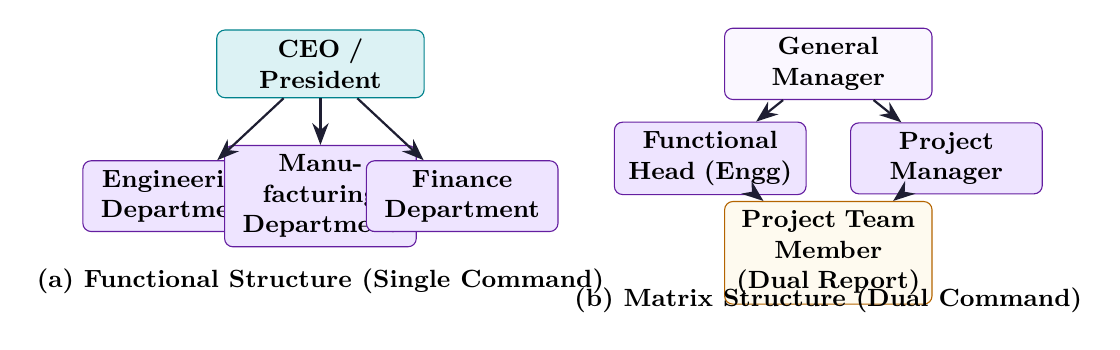
\begin{tikzpicture}[x=1.5cm, y=1.2cm]
  % Functional Structure Diagram (Left)
  \node [block] (ceo) at (1.2, 2.0) {CEO / President};
  \node [sblock] (f1) at (0.0, 0.6) {Engineering\\Department};
  \node [sblock] (f2) at (1.2, 0.6) {Manufacturing\\Department};
  \node [sblock] (f3) at (2.4, 0.6) {Finance\\Department};
  
  \draw [arrow] (ceo) -- (f1);
  \draw [arrow] (ceo) -- (f2);
  \draw [arrow] (ceo) -- (f3);
  \node at (1.2, -0.3) {\small\textbf{(a) Functional Structure (Single Command)}};

  % Matrix Structure Diagram (Right)
  \node [block, fill=hdrpurple!30, draw=mypurple] (mceo) at (5.5, 2.0) {General Manager};
  \node [sblock] (mf) at (4.5, 1.0) {Functional\\Head (Engg)};
  \node [sblock] (pm) at (6.5, 1.0) {Project\\Manager};
  \node [block, fill=hdramber!40, draw=myamber] (team) at (5.5, 0.0) {Project Team\\Member (Dual Report)};

  \draw [arrow] (mceo) -- (mf);
  \draw [arrow] (mceo) -- (pm);
  \draw [arrow] (mf) -- (team);
  \draw [arrow] (pm) -- (team);
  \node at (5.5, -0.5) {\small\textbf{(b) Matrix Structure (Dual Command)}};
\end{tikzpicture}
\end{tcolorbox}

% ===============================================================================
% 4. NATURE AND MODELS OF ORGANIZATIONAL BEHAVIOR
% ===============================================================================
\section{Nature and Scope of Organizational Behavior (OB)}

\textbf{Organizational Behavior (OB)} is an applied behavioral science field that investigates the impact of individuals, groups, and organizational structure on behavior within organizations, for the purpose of applying such knowledge toward improving organizational effectiveness.

\begin{tcolorbox}[defbox, title={Nature of Organizational Behavior}]
  OB is a \textbf{multidisciplinary field} drawing concepts from Psychology (individual level), Sociology \& Social Psychology (group level), and Anthropology \& Political Science (organization system level). It is humanistic, goal-oriented, and science-backed.
\end{tcolorbox}

\subsection{The 5 Fundamental Models of Organizational Behavior}
Organizational culture and managerial philosophy dictate the dominant OB model adopted by a firm:

\par\vspace{6pt}\noindent
\begingroup
\setlength{\tabcolsep}{2.5pt}%
\setlength{\extrarowheight}{3.5pt}%
\renewcommand{\arraystretch}{1.4}%
\footnotesize
\begin{tabularx}{\linewidth}{|>{\raggedright\arraybackslash\bfseries}p{1.9cm}|Y|Y|Y|Y|Y|}
\hline
\multicolumn{1}{|c|}{\textbf{Dimension}} & \multicolumn{1}{c|}{\textbf{Autocratic}} & \multicolumn{1}{c|}{\textbf{Custodial}} & \multicolumn{1}{c|}{\textbf{Supportive}} & \multicolumn{1}{c|}{\textbf{Collegial}} & \multicolumn{1}{c|}{\textbf{System}} \\
\hline
Basis of Model & Power / Authority & Economic resources & Leadership & Partnership & Community \\
\hline
Managerial Orientation & Authority & Money / Benefits & Support & Teamwork & Nurturing \\
\hline
Employee Orientation & Obedience & Security \& Benefit & Job performance & Responsibility & Self-discipline \\
\hline
Employee Psychological Result & Dependence on boss & Dependence on organization & Participation & Self-\allowbreak actualization & Passion \& Commitment \\
\hline
Employee Needs Met & Subsistence (Basic) & Security & Esteem & Self-\allowbreak actualization & Higher-\allowbreak order needs \\
\hline
\end{tabularx}
\endgroup

% ===============================================================================
% QUICK REVISION PAGE
% ===============================================================================
\newpage
\begin{center}
  {\large\bfseries\color{myred} Quick Revision --- Module 1}\\[3pt]
  {\small\color{mydark} Introduction to Organization \& Organizational Behavior $|$ OE-EC804C}
\end{center}
\vspace{-4pt}
\hrule
\vspace{8pt}

\begin{tcolorbox}[formulabox, title={\textbf{Key Concepts and Metrics at a Glance}}]
\renewcommand{\arraystretch}{1.35}
\begin{tabularx}{\linewidth}{>{\raggedright\arraybackslash\bfseries}p{4.5cm} X}
Organization & Social entity consciously coordinated to achieve pre-determined common goals. \\[4pt]
Formal vs Informal Org & Official hierarchical structure vs. spontaneous personal social network (grapevine). \\[4pt]
Fayol's Unity of Command & Principle stating each employee reports to one and only one direct manager. \\[4pt]
Matrix Structure & Dual-authority structure combining functional specialization with project teams. \\[4pt]
OB Field Basis & Multidisciplinary study of individual, group, and structural impact on behavior. \\[4pt]
5 OB Models & Autocratic (Power), Custodial (Security), Supportive (Leadership), Collegial (Teamwork), System (Community). \\
\end{tabularx}
\end{tcolorbox}

\begin{tcolorbox}[defbox, title={\textbf{One-Line Definitions for Exam Revision}}]
  \begin{itemize}[leftmargin=*, itemsep=2pt]
    \item \textbf{Span of Control:} The maximum number of subordinates a manager directly and effectively supervises.
    \item \textbf{Grapevine:} The informal, un official communication channel operating within an organization.
    \item \textbf{Scalar Chain:} The unbroken vertical chain of command from highest executive to lowest worker.
    \item \textbf{Organizational Structure:} The formal framework defining how job tasks are divided, grouped, and coordinated.
  \end{itemize}
\end{tcolorbox}

\begin{tcolorbox}[exambox, title={\textbf{Frequently Asked / Viva Questions}}]
\begin{enumerate}[leftmargin=*, itemsep=4pt]
  \Q{Define an Organization. What are its core components?}{An organization is a consciously coordinated social unit of two or more people working continuously toward common goals. Its core components are People, Structure, Technology, and Environment.}
  
  \Q{Differentiate between Formal and Informal Organizations.}{Formal organizations are officially created by management with rigid hierarchies and written rules. Informal organizations emerge spontaneously among employees to fulfill personal social needs.}
  
  \Q{What is Fayol's Unity of Command principle? Why is it important?}{It states that an employee should receive orders from only one manager. It prevents dual-subordination conflict, confusion, and responsibility shifting.}
  
  \Q{Explain the Matrix Organizational Structure and its major drawback.}{A matrix structure combines functional departments with project teams, creating a dual reporting line. Its main drawback is potential conflict of authority between functional and project managers.}
  
  \Q{What is Organizational Behavior (OB)?}{OB is an applied behavioral science field studying how individuals, groups, and organizational structures influence behavior, aiming to enhance organizational performance.}
  
  \Q{List the 5 primary models of Organizational Behavior.}{Autocratic (power-based), Custodial (money-based), Supportive (leadership-based), Collegial (teamwork-based), and System (community-based).}
  
  \Q{What is Span of Control? Distinguish between Tall and Flat structures.}{Span of control is the number of direct subordinates under a manager. A narrow span produces a Tall structure (many hierarchy levels); a wide span produces a Flat structure (few hierarchy levels).}
  
  \Q{How does Psychology contribute to Organizational Behavior?}{Psychology provides theories on individual behavior, learning, personality, perception, motivation, and job satisfaction.}
  
  \Q{What is the difference between Line and Staff managers?}{Line managers have direct command authority over operational tasks; Staff managers act as advisors providing specialized technical, legal, or HR guidance.}
  
  \Q{Which OB model is oriented towards meeting employee security needs?}{The Custodial model, which relies on economic resources and benefits to fulfill employee safety and financial security needs.}
\end{enumerate}
\end{tcolorbox}

\end{document}
